As with stage ~\ref{step:botcross}, there are two parts to this stage: \begin{enumerate}
	\item Position the corners correctly, see \figref{cornerpos}.
	\item Align the corners, see \figref{all}.
\end{enumerate}
\begin{figure}[h]
	\centering
	\begin{subfigure}[b]{0.3\textwidth}
		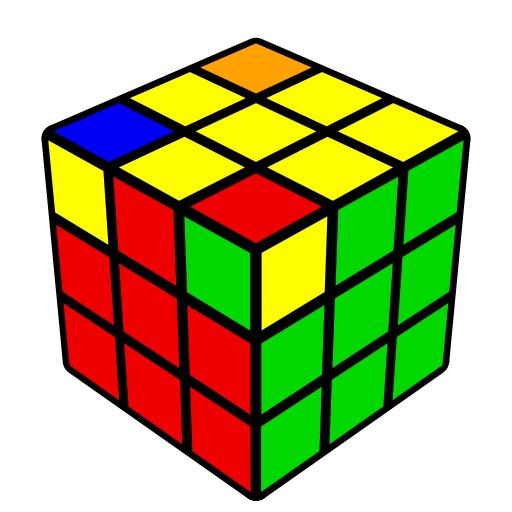
\includegraphics[width=\textwidth]{cornerpos.png}
		\caption{Positioned corners}\label{fig:cornerpos}
	\end{subfigure}
	\begin{subfigure}[b]{0.3\textwidth}
		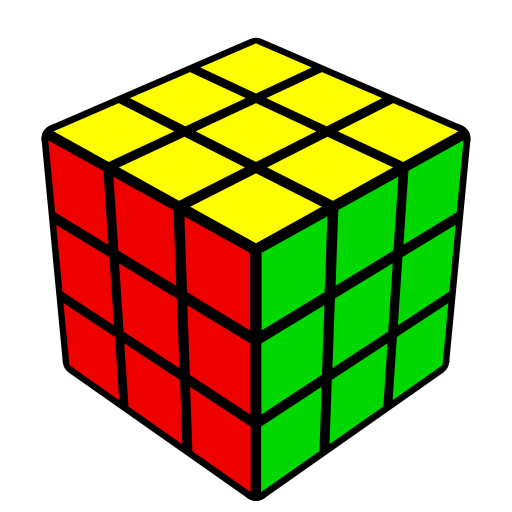
\includegraphics[width=\textwidth]{all.png}
		\caption{Aligned corners}\label{fig:all}
	\end{subfigure}
	\caption{Bottom corners}
\end{figure}	
\begin{enumerate}
	\item Flip the white face to the bottom.
	\item Choose a corner that is already in the correct position. If no such corner is available:\begin{enumerate}
		\item\label{step:cornerfix} Looking at any face of the cube, do \alg{URU'L'UR'U'L}.
		\item Repeat step ~\ref{step:cornerfix} until at least one corner is fixed.
		\item Choose a fixed corner and proceed.
	\end{enumerate}
	\item Orient the cube so that the chosen corner is on the top-right of the front face.
	\item Do \alg{URU'L'UR'U'L} until all corners are fixed.
	\item\label{step:aligncorner} Repeat \alg{R'D'RD} until the top-right corner is correctly aligned.
	\item\label{step:aligncorners} Rotate the entire cube 90\degree to the left. Repeat step ~\ref{step:aligncorner}.
	\item Repeat step ~\ref{step:aligncorners} until all corners are aligned.
	\item Twist the middle layer until the cube is solved.
\end{enumerate}

